
\section{平衡点附近的轨道结构，伯克霍夫范式}
\label{sec:birkhoff-normal-form}

设 $H$ 是在\trEquilibrium{} $z=0$ 附近具有如下形式的\trSmooth{}函数：
\[
H(z)=\sum_{j=1}^{n}\frac{\alpha_j}{2}\bigl(x_j^{2}+y_j^{2}\bigr)+\dotsb=H_2+\dotsb,
\]
那么我们考察\trGroupAction{} $H\circ\tau$，其中 $\tau$ 属于群 $G_1$，即由在%
$z=0$ 附近局部定义的\trSymplectic{}且\trSmooth{}的诸\trDiffeomorphism{}所组成的%
群，这些\trDiffeomorphism{}保持原点与 $H$ 的二次部分 $H_2$ \trInvariant：
\[
G_1=\bigl\{\tau\ \bigm|\ \tau^{*}\omega_0=\omega_0
\quad\text{且}\quad\tau(0)=0,\ d\tau(0)=\id\bigr\}.
\]
目标在于求得一个使 $H\circ\tau$ 呈特别简单形式的\trMapping{} $\tau\in G_1$。我们%
强调，在下文中，二次部分 $H_2$ 是固定的，并且并不假定它是一个%
\textbf{定号\trQuadraticForm}（definite quadratic form）。

\begin{theorem}[\trBirkhoff\trNormalForm]\label{thm:birkhoff-normal-form}
设\trLinear{}\trInvariant{}量 $\alpha=(\alpha_1,\alpha_2,\dotsc,\alpha_n)$ 是 $s$ 阶%
\trNonresonance{}的，即
\[
\langle\alpha,j\rangle\neq0
\qquad\text{对}\quad j\in\Z^{n},\ 0<|j|\leq s,
\]
其中 $|j|=\sum_{\nu=1}^{n}|j_\nu|$。那么存在\trAnalytic{}\trMapping{} $\tau\in G_1$，%
使得
\[
H\circ\tau=F(I_1,\dotsc,I_n)+o_s,
\]
其中 $F$ 是 $n$ 个变量 $I=(I_1,I_2,\dotsc,I_n)$ 的多项式，次数为%
$\bigl[\tfrac{s}{2}\bigr]$，形如
\[
F=\langle\alpha,I\rangle+\frac{1}{2}\langle\beta I,I\rangle+\dotsb,
\]
而 $\beta$ 是一个 $n\times n$ 矩阵。$\R^{2n}$ 上的诸函数 $I_j$ 由
\[
I_j(x,y)=\frac{1}{2}\bigl(x_j^{2}+y_j^{2}\bigr)
\qquad\text{对}\quad 1\leq j\leq n
\]
给出。此外，多项式 $F$ 由 $H$ 唯一确定，并且不依赖于 $\tau\in G_1$ 的选取。
\end{theorem}

因此，$F$ 的系数是 $H$ 的局部\trSymplecticInvariant，称为\trBirkhoffInvariant。%
我们把关于这一\trNormalForm{}意义的讨论搁置到后面，先给出它的证明；该证明%
具有代数的性质。

\begin{proof}
我们迭代地进行，并假设
\[
H=H_2+H_3+\dotsb+H_{m-1}+H_m+\dotsb
\]
已经直到 $m-1$ 阶呈\trNormalForm，其中诸 $H_j$ 是次数为 $j$ 的%
\trHomogeneous{}多项式。我们要寻找一个\trSymplectic\trMapping{} $\tau\in G_1$，它%
不改变已经达到的\trNormalForm，并把 $H\circ\tau$ 直到 $m$ 阶化为\trNormalForm。%
我们取
\[
\tau=\exp\,X_P,
\]
即\trHamiltonianVectorField{} $X_P$ 的时刻 $1$ \trMapping，其中 $P$ 是次数为 $m$%
的\trHomogeneous{}多项式。由于 $\tau$ 属于某个\trHamiltonianVectorField{}的%
\trFlow，它是\trSymplectic{}的，并且形如
\[
\tau(z)=z+J\nabla P(z)+\dotsb,
\]
其中诸点号代表更高阶的项，而且容易算得
\[
H\circ\tau=H_2+H_3+\dotsb+H_{m-1}
+\bigl(H_m-\{H_2,P\}\bigr)+\dotsb.
\]
括号中的多项式是 $m$ 次\trHomogeneous{}的，而括号 $\{\cdot,\cdot\}$ 表示%
\textbf{\trPoissonBracket}（Poisson bracket），它对两个函数 $F$ 与 $G$ 定义如下：
\[
\{F,G\}=\omega\bigl(X_G,\,X_F\bigr).
\]
我们看到，可以借助形如 $\{H_2,P\}$ 的函数来修改 $H$。把次数为 $m$ 的%
\trHomogeneous{}多项式所成的向量空间记作 $V_m$，并令%
$L:V_m\longrightarrow V_m$ 是由 $L(P)=\{H_2,P\}$（对 $P\in V_m$）定义的%
\textbf{\trLinearOperator}（linear operator）。

\begin{lemma}\label{lem:kernel-range-complement}
该\trLinearOperator{}的\trKernel{} $K=K(L)$ 与\textbf{\trRange}（range）%
$R=R(L)$ 是互补的：
\[
V_m=K+R\qquad\text{且}\qquad K\cap R=\{0\}.
\]
此外，若 $\langle\alpha,j\rangle\neq0$ 对 $0<|j|\leq m$ 成立，则当 $m$ 为奇数时%
$K=\{0\}$；若 $m=2k$ 为偶数，则
\[
K=\operatorname{span}\Bigl\{\,I_1^{k_1}\dotsb I_n^{k_n}\ \Bigm|\ %
\sum_{j=1}^{n}k_j=k\,\Bigr\}.
\]
\end{lemma}

因此，\trNormalForm{}恰由 $L$ 的\trKernel{}中的元素组成；我们将把\trNormalForm{}%
所成的集简记为
\[
\mathcal{N}=\bigl\{\,P\ \bigm|\ \{H_2,P\}=0\quad\text{且}\quad%
P\ \text{是一个多项式}\,\bigr\}.
\]

\begin{proof}[\trhLemma{}的\trhProof]
为了在 $V_m$ 中把 $L$ \trDiagonal{}化，我们转入复变量，并选取%
\trSymplecticCoordinates
\begin{align*}
\xi_\nu &=\tfrac{1}{\sqrt{2}}\ \bigl(x_\nu+i\,y_\nu\bigr)\\
\eta_\nu &=\tfrac{1}{\sqrt{2}}\ \bigl(y_\nu+i\,x_\nu\bigr)
\end{align*}
使得 $\xi_\nu\eta_\nu=\tfrac{i}{2}\bigl(x_\nu^{2}+y_\nu^{2}\bigr)$，而%
$H_2=\tfrac{1}{i}\sum_{\nu=1}^{n}\alpha_\nu\bigl(\xi_\nu\eta_\nu\bigr)$。从而
\[
L\bigl(\xi^{k}\eta^{\ell}\bigr)=\bigl\{H_2,\ \xi^{k}\eta^{\ell}\bigr\}
=\frac{1}{i}\,\bigl\langle\alpha,\ \ell-k\bigr\rangle\,\xi^{k}\eta^{\ell}.
\]
我们已简记 $\langle\alpha,\ell-k\rangle=\sum_{\nu=1}^{n}\alpha_\nu(\ell_\nu-k_\nu)$。%
若 $P\in V_m$，则
\[
P=\sum_{|k|+|\ell|=m}p_{k\ell}\,\xi^{k}\eta^{\ell}
\]
可分解为 $P=P^{K}+P^{N}$，其中 $P^{K}\in K(L)$ 含有使%
$\langle\alpha,k-\ell\rangle=0$ 的诸系数 $p_{k\ell}$，而 $P^{N}$ 含有使%
$\langle\alpha,k-\ell\rangle\neq0$ 的诸系数。在 $m$ 阶\trNonresonance{}的情形，%
我们有 $\langle\alpha,\ell-k\rangle=0$ 当且仅当 $k=\ell$。此时，$K(L)$ 由形如%
$\xi^{k}\eta^{k}=(\xi\eta)^{k}$ 的单项式组成，而这些单项式在原坐标下正是形如%
$I^{k}=I_1^{k_1}\dotsb I_n^{k_n}$ 的单项式，即为所求。至此引理证毕。
\end{proof}

鉴于该引理，容易确定所要的\trMapping{} $\tau$。把 $H_m=H_m^{R}+H_m^{K}$ 分解成%
$H_m^{R}\in R(L)$ 与 $H_m^{K}\in K(L)$，使得
\[
H_m-\{H_2,P\}=H_m^{R}+H_m^{K}-\{H_2,P\},
\]
我们选取多项式 $P$ 作为 $\{H_2,P\}-H_m^{R}=0$ 的一个解。此时，函数 $H\circ\tau$%
直到 $m$ 阶呈\trNormalForm。把刚才构造的\trMapping{}记作 $\tau=\tau_m$，我们看到，%
把 $H$ 直到 $s$ 阶化为\trNormalForm{}的那个所要\trMapping{}，作为诸\trMapping{}的%
一个复合被迭代地求得：
\[
\tau_s\circ\tau_{s-1}\circ\dotsb\circ\tau_3,
\]
其中 $\tau_j\in G_1$。剩下只需证明\trNormalForm{}的唯一性。这由下一个引理得出。

\begin{lemma}\label{lem:normal-form-uniqueness}
设 $\alpha$ 是 $s$ 阶\trNonresonance{}的。若 $\tau_1$, $\tau_2\in G_1$ 满足
\begin{align*}
H\circ\tau_1 &= F+o_s,\\
H\circ\tau_2 &= \hat{F}+o_s,
\end{align*}
其中 $F$ 与 $\hat{F}$ 是呈\trNormalForm{}的 $s$ 次多项式，即%
$F$, $\hat{F}\in\mathcal{N}$，则
\begin{align*}
&\text{(i)}\qquad F=\hat{F},\\
&\text{(ii)}\qquad \tau=\tau_1^{-1}\circ\tau_2=\exp\,X_P+o_s,
\end{align*}
其中 $P=P_3+\dotsb+P_s$ 是一个 $s$ 次多项式，且 $P\in\mathcal{N}$。
\end{lemma}

\begin{proof}
\let\qed\relax%
显然，只需取已呈\trNormalForm{}的 $H=F$ 即可，于是
\[
\hat{F}\circ\tau=F+o_s.
\]
我们必须证明 $\hat{F}=F$，并且 $\tau\in G_1$ 满足 (ii)。再次按归纳法进行，我们%
假设
\[
P=P_3+\dotsb+P_{m-1}+P_m+\dotsb+P_s
\]
其中 $P_j\in\mathcal{N}$（$3\leq j\leq m-1$），并证明也有 $P_m\in\mathcal{N}$。%
为了确定 $m$ 阶的项，我们对两个函数 $H$, $G$ 使用公式
\[
H\circ\exp\,X_G=H+\{H,G\}+\bigl\{\{H,G\},G\bigr\}+\dotsb
\]
它由 $H\circ\exp\,tX_G$ 在 $t=0$ 处关于 $t$ 的\trTaylor{}展开得出。现在，若%
$\hat{F}=H_2+\hat{F}_3+\dotsb+\hat{F}_s$，类似地 $F=H_2+F_3+\dotsb+F_s$，我们发现
\[
\hat{F}_m+\bigl\{H_2,\ P_m\bigr\}+A_m=F_m,
\]
其中，由归纳假设，$A_m$ 是 $\mathcal{N}$ 中元素的若干\trPoissonBracket{}之和。由于%
$\mathcal{N}$ 是一个子代数，我们有 $A_m\in\mathcal{N}$\footnote{原书印作「$A_m\subset\mathcal{N}$」，疑为「$A_m\in\mathcal{N}$」之误：$A_m$ 是诸泊松括号之和，为一多项式（元素）而非子集，此处径改。——译者注}，因此
\[
\bigl\{H_2,\ P_m\bigr\}\in\mathcal{N}.
\]
鉴于前一引理，我们得出 $\{H_2,P_m\}=0$，从而 $P_m\in\mathcal{N}$。归纳步骤至此%
完成，于是我们可以假定 $P\in\mathcal{N}$。代数 $\mathcal{N}$ 直到 $s$ 阶是\trAbelian{}的，%
因为我们假定\trNonresonance{}条件对 $\alpha$ 直到 $s$ 阶成立；这由%
\cref{lem:kernel-range-complement} 得出。因此 $\{\hat{F},P\}=0$，从而
\[
\hat{F}\circ\tau=\hat{F}\circ\exp\,X_P=\hat{F}.
\]
由于 $\hat{F}\circ\tau=F+o_s$，我们得出 $\hat{F}=F$，正如引理所断言。至此引理证毕。
\end{proof}

从而，\trBirkhoff{}定理也随之得证。
\end{proof}

从动力学的观点来看，\trBirkhoff\trNormalForm{}的意义在于：\trSymplectic{}变换%
$\tau$ 使\trHamiltonianSystem{}在\trEquilibrium{}的一个小\trNeighborhood{}内%
可积，当然，只是直到更高阶的诸项 $o_s$ 为止。的确，暂时舍去更高阶的项，%
相应的\textbf{\trIntegrableSystem}（integrable system）便由\trHamiltonianFunction
\[
F(I_1,I_2,\dotsc,I_n)
\]
在 $\R^{2n}$ 上定义，它是 $n$ 个函数 $I_j(x,y)=\frac{1}{2}\bigl(x_j^{2}+y_j^{2}\bigr)$%
的多项式。这些函数是 $F$ 的 $n$ 个\trFirstIntegral，此外它们%
还两两\textbf{\trInvolution}（in involution），即 $\{I_i,I_j\}=0$。于是，%
\trHamiltonianEquation{} $X_F$ 的解便可以借助于这些\trFirstIntegral{}而显式地、并对一切时刻给出。%
从 $\R^{2n}$ 中除去坐标轴，%
并按
\[
y_\nu+i\,x_\nu=\sqrt{2r_\nu}\,e^{i\vartheta_\nu}
\]
（$\nu=1,2,\dotsc,n$，$r_\nu>0$，而 $\vartheta_\nu$ 取模 $2\pi$）引入%
\trSymplectic{}\textbf{\trPolarCoordinates}（polar coordinates），便有
\[
\sum_{j=1}^{n}dy_j\wedge dx_j=\sum_{j=1}^{n}d\vartheta_j\wedge dr_j
\]
而\textbf{\trSymplectic\trPhaseSpace}（symplectic phase space）就成为
\[
T^{n}\times\Omega,\qquad\Omega=(\R^{+})^{n}\subset\R^{n}.
\]
由于 $r_\nu=I_\nu$，变换后的\trHamiltonianFunction{}便由%
$F(r_1,r_2,\dotsc,r_n)$ 给出，并且不依赖于诸角变量%
$\vartheta_1,\dotsc,\vartheta_n$。\trVectorField
\[
X_F:\quad
\begin{cases}
\dot{\vartheta}=\dfrac{\partial}{\partial r}\,F(r),\\[8pt]
\dot{r}=-\dfrac{\partial}{\partial\vartheta}\,F(r)=0
\end{cases}
\]
的\trFlow{} $\varphi^{t}(r)$ 可以立即读出：
\[
\varphi^{t}(\vartheta,r)=\bigl(\vartheta+t\omega,\ r\bigr).
\]
所谓的\textbf{\trFrequencyVector}（frequency vector）$\omega$ 由
\[
\omega=\omega(r)=\frac{\partial}{\partial r}\,F(r)\in\R^{n}
\]
定义。

该\trFlow{}使每一个\textbf{\trTorus}（torus）%
$T^{n}\times\{r\}\subset T^{n}\times\Omega$ 保持\trInvariant，而且在此\trTorus{}上，%
该\trFlow{}是由诸频率 $\omega(r)$ 所定义的\trLinear\trKronecker\trFlow。与%
\trLinear{}情形相反，这些频率一般依赖于诸\trFirstIntegral{} $r$。例如，若 $\det\beta\neq0$%
（$\beta$ 如\trNormalForm{}中所定义），便是这种情形。在原坐标下，诸解是%
\trQuasiPeriodic{}的，并表示为
\[
y_\nu(t)+i\,x_\nu(t)=\sqrt{2r_\nu}\,e^{i\left(\vartheta_\nu+t\,\omega_\nu(r)\right)},
\]
其中 $y_\nu(0)+i\,x_\nu(0)=\sqrt{2r_\nu}\,e^{i\vartheta_\nu}$。

作为附带评注，我们指出：若诸 $\alpha_j$ 对每一阶都\trNonresonance，即%
\textbf{\trRationallyIndependent}（rationally independent），那么按%
\trNormalForm{}证明中那样进行，我们便归纳地求得一个呈\textbf{\trFormalPowerSeries}%
（formal power series）\trMapping{}形状的\trSymplectic\trMapping{}%
$\tau$，它把\trHamiltonianFunction{} $H$ 化为可积形式 $H\circ\tau=P_\infty(I)$。%
它借助\trFirstIntegral{} $I=(I_1,I_2,\dotsc,I_n)$ 中的一个\trFormalPowerSeries{}给出，%
表示 $H$ 在 $0$ 处的无穷多个\trSymplecticInvariant。这是一个纯代数的论断。若%
$H$ 是\trAnalytic{}的，而且 $\tau$ 可以选取得\trConverge，则\trHamiltonianSystem{}%
便可以在\trEquilibrium{}附近被显式解出。然而众所周知，$\tau$ 的\trDivergence{}%
才是典型情形。这由 C.~L.~\trSiegel{}于 1954 年证明 [195]。乍一看，%
\trNormalForm{}对于研究%
\trHamiltonianSystem{}在\trEquilibrium{}附近的\trOrbit{}结构似乎因此毫无用处。%
然而情况并非如此。若把 $X_H$ 看作\trIntegrableSystem{} $X_F$ 在\trEquilibrium{}附近的一个%
\trPerturbation，\trBirkhoff{}定理中的\trNormalForm{}便能得到非常有效的利用。%
的确，\trPerturbation{}方法使我们能够把\trIntegrableSystem{} $X_F$ 的某些动力学现象%
\trContinuation{}到原点附近的完整系统 $X_H$，下面我们将对此予以例释，尽管不%
给出证明。

设 $\alpha$ 是 $s=4$ 阶\trNonresonance{}的。鉴于\trBirkhoff{}定理，在经过一个%
\trNonlinear\trSymplectic{}变换 $\tau\in G_1$ 之后，我们可以假定%
\trHamiltonianFunction{}在 $z=0$ 附近形如
\begin{align*}
H(z) &= F(I)+o_4(z)\\
F(I) &= \langle\alpha,I\rangle+\frac{1}{2}\langle\beta I,I\rangle.
\end{align*}
假定系统 $X_H$ 是\trNonlinear{}且\trNondegenerate{}的，即对\trSymplecticInvariant{}%
$\beta$ 提出要求
\[
\det\beta\neq0,
\]
那么容易验证：\trEquilibrium{}的每一个去心\trNeighborhood{}%
$0<|z|<\varepsilon$ 都含有\trIntegrableSystem{} $X_F$ 的一条\trPeriodicSolution，%
从而 $z=0$ 是 $X_F$ 的诸\trPeriodicSolution{}的一个\textbf{\trAccumulationPoint}%
（cluster point）。这些解的%
\trPeriodic{}趋于无穷。同样的论断对于以完整系统 $X_H$ 代替 $X_F$ 也成立，这已由%
G.~\trBirkhoff{}与\trLewis{}于 1933 年证明 [27]。关于证明，我们参考%
J.~\trMoser{} [164]，他给出了一个更为一般的结果之证明。

此外，若 $X_H$ 还是充分\trSmooth{}的（例如 $H\in C^{\ell}$，$\ell=2n+3$），那么%
著名的 K.A.M.~理论\footnote{译注：K.A.M.~系\trKolmogorov、\trArnold{}与%
\trMoser{}三人姓氏的首字母缩写。}便可以应用，%
并使我们得以更深入地洞察 $X_H$ 在\trEquilibrium{}附近的\trOrbit{}结构。尽管%
可积性在\trPerturbation{}之下遭到破坏，我们仍可断言：许多 $r$ 很小的、在可积%
系统 $X_F$ 之下\trInvariant{}的\trTorus{} $T^{n}\times\{r\}$，可以作为在\trFlow{}%
$X_H$ 之下\trInvariant{}的\trEmbedding{}\trLagrange{}\trTorus{}%
$T_r=\varphi\bigl(T^{n}\times\{r\}\bigr)$ 而\trContinuation。在诸\trTorus{} $T_r$ 上，%
\trFlow{}是由 $\dot{\vartheta}=\omega(r)$ 给出的\trKronecker\trFlow，于是 $T_r$ 被%
$X_H$ 的具有频率 $\omega(r)$ 的诸\trQuasiPeriodic{}解所覆盖。此外，这些%
\trInvariant\trTorus{}在\trPhaseSpace{}中填出一个\trLebesgue{}\trMeasure{}相对%
很大的\trCantor{}集。

这些证明本质上是分析性的，并且由于\textbf{\trSmallDenominator}（small denominator）%
的困难而十分精微。这一困难在六十年代被\trKolmogorov{} [128]、\trArnold{} [7, 8]%
与 J.~\trMoser{} [159] 所克服。关于近期的表述与文献，我们参考%
J.~\trPoschel{} [178]；另见 [189]。

结果表明，由 K.A.M.~理论构造的诸\trInvariant\trTorus{}位于\trPeriodicOrbit{}所成%
集合的\textbf{\trClosure}（closure）之中。这一观察引出下述关于\trEquilibrium{}%
附近\trPeriodicOrbit{}的局部存在性论断，其证明可在 [56] 中找到。

\begin{theorem}\label{thm:local-existence-periodic-orbits}
设 $H\in C^{\ell}$（$\ell\geq2n+3$）且满足 $\alpha$ 的 $s=4$ 阶\trNonresonance{}%
条件。设该系统是\trNonlinear{}的，即要求 $\det\beta\neq0$。若 $S_\varepsilon$%
表示含于以\trEquilibrium{}为中心、半径为 $\varepsilon$ 的开\trBall{}%
$B(\varepsilon)$ 之内的诸\trPeriodicSolution{}所成集合的\trClosure，则
\[
m\bigl(B(\varepsilon)\setminus S_\varepsilon\bigr)
=O\bigl(\sqrt{\varepsilon}\bigr)\,m\bigl(B(\varepsilon)\bigr),
\]
其中 $m$ 表示\trLebesgue{}\trMeasure。
\end{theorem}

这些\trPeriodicSolution，以及\trEquilibrium{}附近的诸\trQuasiPeriodic{}解，只需对%
$H$ 在 $z=0$ 处的有限多个局部\trSymplecticInvariant{}假定有限多个不等式，便能%
建立。\trLinear{}\trInvariant{}量的高阶\textbf{\trResonance}（resonance）由于所%
设定的\trNonlinear{}性而不起任何作用。这是\trHamiltonian{}力学中的一种典型%
现象。另一方面，应当记得，所应用的分析方法对系统要求大量的\trDerivative。

迄今所描述的\trEquilibrium{}附近的诸\trOrbit，都是借助\trPerturbation{}方法从%
\trBirkhoff\trNormalForm{}的可积部分的相应\trOrbit{}推得的。一般而言，还%
存在着性质上迥然不同的其他\trOrbit，它们与可积部分不相容，而其存在正好解释了%
\trNormalForm{}的\trDivergence。这一点由 V.~\trArnold{}与 A.~\trAvez{}在其著作 [12]%
（1968 年）中的著名略图作了最好的例示。该图展示了 $\R^{2}$ 平面内一个%
\textbf{\trStable\trFixedPoint}（stable fixed point）附近\trNonlinear\trSymplectic%
\trMapping{} $\varphi$ 的\trOrbit{}结构的复杂性。这样的\trMapping{}得以产生，%
例如是作为三维\trEnergySurface{}上的\trHamiltonianSystem{}在一条%
\trStable\trPeriodicOrbit{}附近的\textbf{\trTransversalSection\trMapping}%
（transversal section map）。与其对一切时刻研究邻近的\trOrbit，人们同样可以%
径直研究其\trSection{}\trMapping{}的迭代。

居于中间的\trFixedPoint{} $0$ 被一些接近于\trCircle{}的\trSmooth\trCurve{}所%
环绕，这些\trCurve{}在\trMapping{} $\varphi$ 之下\trInvariant。它们是%
J.~\trMoser{}于 1962 年发现的 [159]。这些\trCurve{}填出一个\trMeasure{}相对很大的%
\trCantor{}集，反映出该\trMapping{}在\trFixedPoint{}附近的可积\trApproximation。%
在这些\trCurve{}之间，人们\trGeneric{}地会发现\trElliptic{}与\trHyperbolic\trPeriodic{}点的%
\trOrbit。此外，由\trHyperbolic\trPeriodic{}点发出的\textbf{\trStableManifold}%
（stable manifold）与%
\textbf{\trUnstableManifold}（unstable manifold）确实\trTransversal{}地相交于%
所谓的\trHomoclinic{}点。众所周知，这些点会使 $\varphi$ 的\trOrbit{}结构变得%
相当复杂，并破坏可积图景。特别地，它们给出\trInvariant{}的\trHyperbolic{}集，%
在其上，\trMapping{}的迭代可以借助\trTopology{}\trBernoulli{}移位从统计上%
加以描述。人们甚至能够证明，\trElliptic\trFixedPoint{}是这类\trHomoclinic{}点的%
一个\trAccumulationPoint。此外，对于该\trMapping{}的更高次迭代，这幅图景在椭圆%
\trPeriodicOrbit{}附近重演，如此等等。图中的虚线表示晚近发现的\trMather{}集，%
关于它们我们参考 J.~\trMather{} [151]。图中诸\trHomoclinic\trOrbit{}的%
\trGeneric{}存在性由%
E.~\trZehnder{}于 1973 年在 [230] 中建立。关于一个改进了的现代版本，我们指出%
C.~\trGenecand{} [104]（1991）；进一步的文献有 A.~\trChenciner{} [49] 与%
J.~\trMoser{} [162]。


\noindent\begin{minipage}{\linewidth}
\centering
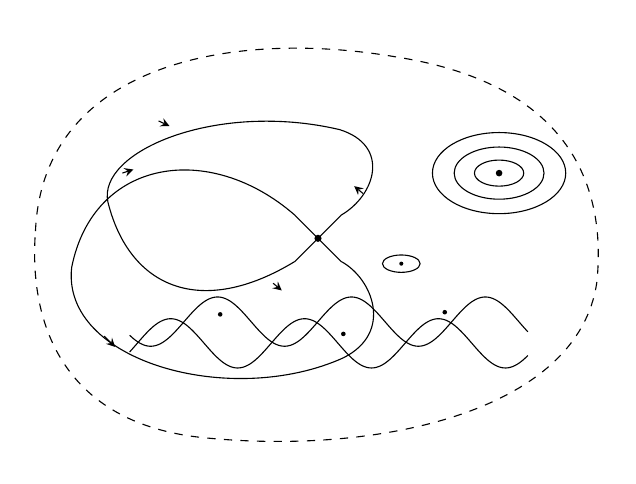
\begin{tikzpicture}[>=stealth,scale=0.92]
  \fill (0,0) circle (1.4pt);
  \draw (-0.32,0.32) -- (0.32,-0.32);   %
  \draw (-0.32,-0.32) -- (0.32,0.32);   %
  \draw (-0.32,0.32) .. controls (-1.5,1.35) and (-3.1,1.1) .. (-3.4,-0.4)
        .. controls (-3.55,-1.7) and (-1.2,-2.35) .. (0.35,-1.65)
        .. controls (1.05,-1.3) and (0.75,-0.55) .. (0.32,-0.32); %
  \draw (-0.32,-0.32) .. controls (-1.6,-1.1) and (-2.6,-0.7) .. (-2.9,0.5)
        .. controls (-3.05,1.2) and (-1.4,1.9) .. (0.3,1.5)
        .. controls (1.0,1.28) and (0.8,0.6) .. (0.32,0.32);   %
  \draw[domain=-2.6:2.9,samples=220,smooth] plot (\x,{0.34*sin(3.4*\x r)-1.15});
  \draw[domain=-2.6:2.9,samples=220,smooth] plot (\x,{0.34*sin(3.4*\x r+2.2 r)-1.45});
  \fill (-1.35,-1.05) circle (0.9pt);   %
  \fill (0.35,-1.32) circle (0.9pt);
  \fill (1.75,-1.02) circle (0.9pt);
  \fill (2.5,0.9) circle (1.3pt);
  \draw (2.5,0.9) ellipse (0.34 and 0.18);
  \draw (2.5,0.9) ellipse (0.62 and 0.36);
  \draw (2.5,0.9) ellipse (0.92 and 0.56);
  \draw (1.15,-0.35) ellipse (0.26 and 0.12);
  \fill (1.15,-0.35) circle (0.8pt);
  \draw[dashed] (-3.9,0.1) .. controls (-3.8,2.4) and (-1.2,2.9) .. (1.1,2.5)
        .. controls (3.3,2.15) and (4.0,0.9) .. (3.85,-0.6)
        .. controls (3.6,-2.4) and (0.8,-3.0) .. (-1.6,-2.75)
        .. controls (-3.5,-2.55) and (-4.0,-1.2) .. (-3.9,0.1);
  \draw[->] (-2.2,1.62) -- (-2.05,1.55);
  \draw[->] (-2.95,-1.35) -- (-2.8,-1.5);
  \draw[->] (-0.62,-0.62) -- (-0.5,-0.72);
  \draw[->] (0.62,0.62) -- (0.5,0.72);
  \draw[->] (-2.7,0.9) -- (-2.55,0.95);
\end{tikzpicture}

图 1.5
\end{minipage}

上图展示了\trHamiltonianSystem{}的\trOrbit{}结构的复杂性，并且特别表明：%
长时间行为迥异的诸\trOrbit，一般而言，确实并肩共存。这一现象使得借助求解%
\trCauchy{}\trInitialValueProblem{}来研究长时间行为成为一项无望的任务。相比之下，%
我们以后要处理的\trPeriodicSolution{}的存在性问题，则引出一个以%
\trVariationalPrinciple{}为特征的\textbf{\trBoundaryValueProblem}（boundary value problem）。

上面所描述的局部存在性结果本质上是分析性的。相比之下，第 4 章的目标在于%
求出整体的\trPeriodicSolution。类似于\trEquilibrium{}附近的情形，一条%
\trPeriodicSolution{}附近的\trOrbit{}结构也可以借助一个\trBirkhoff\trNormalForm{}%
来研究。这一\trNormalForm{}表示该系统在这条\trPeriodicSolution{}局部附近的%
一个可积\trApproximation，其中\trLinear{}\trInvariant{}量现在是该%
\trPeriodicOrbit{}的\trFloquet{}乘子。应当提到，虽然求出这些%
整体\trPeriodicSolution{}所用的定性方法十分有力，但它们尚不足以获得关于这些%
\trPeriodicSolution{}的\trBirkhoffInvariant{}的信息。尽管如此，重要的是要记住：%
\trHamiltonianSystem{}的一条单一\trPeriodicOrbit{}携带着关于其附近一个非常%
丰富的\trOrbit{}结构的潜在信息，其中包括许多具有更大\trPeriodic{}的其他%
\trPeriodicOrbit、诸\trQuasiPeriodic{}解以及\trHyperbolic{}现象。
